\documentclass[tikz, letterpaper,12pt]{article}

\usepackage{geometry}
\usepackage{pslatex}
\usepackage{fancyhdr}
\usepackage{graphicx}
\usepackage{color}
\usepackage{subcaption}
\usepackage{float}
\usepackage{tikz}
\usepackage{setspace}
\geometry{ margin = 1.0in }

\usepackage{listings}
\usepackage{color}

\usepackage[fleqn]{mathtools}
\DeclarePairedDelimiter\ceil{\lceil}{\rceil}
\DeclarePairedDelimiter\floor{\lfloor}{\rfloor}

\definecolor{dkgreen}{rgb}{0,0.6,0}
\definecolor{gray}{rgb}{0.5,0.5,0.5}
\definecolor{mauve}{rgb}{0.58,0,0.82}

\lstset{frame=tb,
  language=Java,
  aboveskip=3mm,
  belowskip=1mm,
  showstringspaces=false,
  columns=flexible,
  basicstyle={\small\ttfamily},
  numbers=none,
  numberstyle=\tiny\color{gray},
  keywordstyle=\color{blue},
  commentstyle=\color{dkgreen},
  stringstyle=\color{mauve},
  breaklines=true,
  breakatwhitespace=true,
  tabsize=3
}

\usepackage{amssymb, amsthm, bm, nicefrac}

\newcommand{\xto}[1]{\xrightarrow{#1}}
\newcommand{\NN}{\mathbb{N}}
\newcommand{\ZZ}{\mathbb{Z}}
\newcommand{\QQ}{\mathbb{Q}}
\newcommand{\RR}{\mathbb{R}}
\newcommand{\CC}{\mathbb{C}}
\newcommand{\abs}[1]{\left|#1\right|}
\newcommand{\norm}[1]{\left\|#1\right\|}
\newcommand{\normal}{\trianglelefteq}
\renewcommand{\qedsymbol}{\rule{0.7em}{0.7em}}

\newcommand{\aaa}[1]{\hspace{0.65cm}\parbox[t]{15.3cm}{#1}}
\newcommand{\aab}[1]{\hspace{1.15cm}\parbox[t]{15.0cm}{#1}}
\newcommand{\aac}[1]{\hspace{1.65cm}\parbox[t]{15.0cm}{#1}}
\newcommand{\aad}[1]{\hspace{2.15cm}\parbox[t]{15.0cm}{#1}}
\newcommand{\aaA}[2]{\hspace{0.5cm} {\tikz[overlay] \draw (0.1, -0.1) -- (0.1, #1 * -1.5em + 0.6em);} \parbox[t]{15.0cm}{#2}}
\newcommand{\aaB}[2]{\hspace{1.0cm} {\tikz[overlay] \draw (0.1, -0.1) -- (0.1, #1 * -1.5em + 0.6em);} \parbox[t]{15.0cm}{#2}}
\newcommand{\aaC}[2]{\hspace{1.5cm} {\tikz[overlay] \draw (0.1, -0.1) -- (0.1, #1 * -1.5em + 0.6em);} \parbox[t]{15.0cm}{#2}}
\newcommand{\aaD}[2]{\hspace{2.0cm} {\tikz[overlay] \draw (0.1, -0.1) -- (0.1, #1 * -1.5em + 0.6em);} \parbox[t]{15.0cm}{#2}}
\newcommand{\xxx}{\par\vspace{0.1cm}}

%%% TODO modify these variables %%%
\def\homeworknum{2}
\def\namex{Param Somane}
\def\accessx{pss5256}
%%%%

\pagestyle{fancy}
\lhead{{\bf CMPSC 465 Fall 2020}}
\chead{{\bf Writing Assignment~\homeworknum}}
\rhead{{\bf September 27, 2020}}

\newcounter{problemid}\stepcounter{problemid}
\def\newproblem{\vspace*{0.01cm}{\bf Problem~\arabic{problemid}\stepcounter{problemid}}\hfill\fbox{\parbox{0.16\textwidth}{\bf Points:}}\par}

\setlength\parindent{0em}
\setlength\parskip{8pt}
\setlength{\fboxsep}{6pt}
\newtheorem{definition}{Definition}
\newtheorem{property}{Property}
\newtheorem{claim}{Claim}
\newtheorem{fact}{Fact}
\newtheorem{corollary}{Corollary}
\newtheorem{lemma}{Lemma}

\makeatletter
\newenvironment{proof*}[1][\proofname]{\par
  \pushQED{\qed}%
  \normalfont \partopsep=\z@skip \topsep=\z@skip
  \trivlist
  \item[\hskip\labelsep
        \itshape
    #1\@addpunct{.}]\ignorespaces
}{%
  \popQED\endtrivlist\@endpefalse
}
\makeatother

\begin{document}

\framebox[\textwidth]{
	\parbox{0.96\textwidth}{
		\parbox{0.08\textwidth}{\bf Name:}\parbox{0.65\textwidth}{\namex}\parbox{0.12\textwidth}{\bf Access ID:}\parbox{0.14\textwidth}{\accessx}
	}
}

%% your solutions %%%
\newproblem
1. The lowest point $p^*\in C_1\cup C_2$ is $p_1$ since it has the smallest y-coordinate.

2. $C_1'=(p_1,p_3,p_5,p_9,p_{10})$ and it is clear from Figure 1 below that the points in $C_1'$ are sorted in increasing angle with respect to $p^*$.

3. We have the points in $C_2$ with the smallest and largest angle with respect to $p^*$ as $p_R=p_7$ and $p_L=p_6$ respectively. Thus, we obtain $C_{2a}=(p_7,p_8,p_{11},p_4)$ and $C_{2b}=(p_2,p_6)$. Both $C_{2a}$ and $C_{2b}$ are sorted in increasing order of angles with respect to $p^*$.

4. $C_2'=(p_7,p_8,p_2,p_{11},p_4,p_6)$, which is obtained by merging $C_{2a}$ and $C_{2b}$.

5. $C'=(p_1,p_3,p_5,p_7,p_8,p_2,p_9,p_{11},p_4,p_{10},p_6)$. All the points in $C'$ are sorted in order of increasing angles with respect to $p^*=p_1$.
\begin{figure}[H]
\centering
    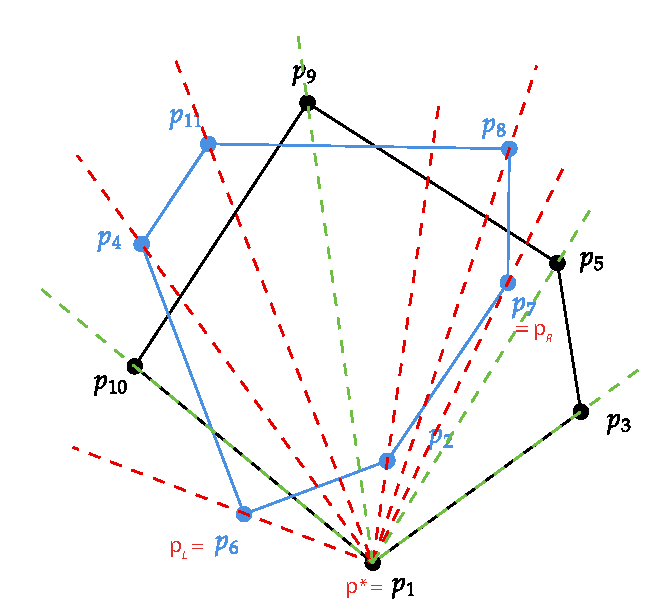
\includegraphics[scale=1.3]{WA2/images/convex-hull.pdf}
    \caption{Pre-processing stage of $CHDC(C')$.}
\end{figure}
6. The stack operations resulting from running Graham-Scan-Core($C'$) are as follows:

push $p_1$; $Stack(S)=(p_1)\\$
push $p_3$; $S=(p_1,p_3)\\$
push $p_5$; $S=(p_1,p_3, p_5)\\$
For $p_7$: push $p_7$; $S=(p_1,p_3, p_5,p_7)\\$
For $p_8$: push $p_8$; pop $p_7$; $S=(p_1,p_3,p_5,p_8)\\$
For $p_2$: push $p_2$; $S=(p_1,p_3,p_5,p_8, p_2)\\$
For $p_9$: push $p_9$; pop $p_2$; $S=(p_1,p_3,p_5,p_8, p_9)\\$
For $p_{11}$: push $p_{11}$; $S=(p_1,p_3,p_5,p_8, p_9, p_{11})\\$
For $p_4$: push $p_4$; $S=(p_1,p_3,p_5,p_8, p_9, p_{11}, p_4)\\$
For $p_{10}$: push $p_{10}$; $S=(p_1,p_3,p_5,p_8, p_9, p_{11}, p_4, p_{10})\\$
For $p_6$: push $p_6$; $S=(p_1,p_3,p_5,p_8, p_9, p_{11}, p_4, p_{10}, p_6)$

Hence, we obtain the convex hull of $C'$ as $CH(C') = (p_1,p_3,p_5,p_8, p_9, p_{11}, p_4, p_{10}, p_6).$

\newproblem

1. After running the DFS (with timing) algorithm on the given directed graph $G=(V,E)$, we obtain $postlist = (v_8,v_7,v_1,v_2,v_4,v_6,v_3,v_5)$. The $pre$ and $post$ numbers of all vertices have been provided in Figure 2 below.
\begin{figure}[H]
\centering
    \includegraphics[scale=1.55]{WA2/images/dfs.jpg}
    \caption{The $[pre,\,post]$ interval for each vertex is marked next to each vertex.}
\end{figure}
\newpage
2. The meta graph for $G$ is given in Figure 3 below.
\begin{figure}[H]
\centering
    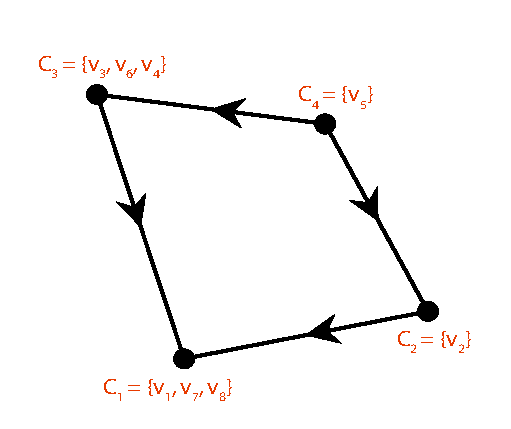
\includegraphics[scale=1.3]{WA2/images/meta.pdf}
    \caption{Meta graph $G^M=(V^M,E^M)$ of $G$.}
\end{figure}

3. Since $G^M$ is a DAG, it can be linearized. $X=(C_4,C_2,C_3,C_1)$ gives a linearization of $G^M$.

4. The meta graph $G^M$ has only $C_4$ as a source and $C_1$ as a sink. Hence, in any linearization of $G^M$, $C_4$ must occur in the first position and $C_1$ must be in the last position. The middle two elements can be permuted in either order as there is no edge connecting them; ergo, the meta-graph has only two possible linearizations, namely $G^M_1=(C_4,C_2,C_3,C_1)$ and $G^M_2=(C_4,C_3,C_2,C_1)$.

\newproblem
We claim that a DAG $G$ has a unique linearization if and only if the consecutive vertices in its linearization have successive edges connecting them.
\begin{lemma}
Let $G=(V,E)$ be a DAG and let $X=(v_{i_1},\cdots,v_{i_n})$ be a linearization of $G$ with $n=|V|$. Then $X$ is the unique linearization of $G$ if and only if $\;\forall k\in\{1,2,\cdots,n-1\},\, (v_{i_k},v_{i_{k+1}})\in E$.
\begin{proof}
We first prove the forward implication.

$\Longrightarrow :$
Suppose $\exists k\in\{1,2,\cdots,n-1\}$ such that $(v_{i_k},v_{i_{k+1}})\notin E$.
Then we have an alternate linearization $X'=(v_{i_1},\cdots,v_{i_{k-1}},v_{i_{k+1}},v_{i_k},v_{i_{k+2}},\cdots,v_{i_n})$ of $G$ because the linearization property is induced from $X$ for vertices other than $v_{i_k}$ and $v_{i_{k+1}}$ and since these two vertices are not connected by an edge, their ordering relative to each other is irrelevant and so they too satisfy the linearization property with the other vertices in $X'$. Hence, $X$ is not the unique linearization of $G$.

$\Longleftarrow :$ For the other direction, suppose, toward a contradiction, that $\forall k\in\{1,2,\cdots,n-1\},\, (v_{i_k},v_{i_{k+1}})\\\in E$ but $X$ is not a unique linearization of $G$. Let $X'$ be another linearization of $G$ that is distinct from $X$. Hence $\exists k\in\{1,\cdots,n-1\}$ such that $v_{i_{k+1}}$ is before $v_{i_k}$ in $X'$ because otherwise , if $v_{i_k}$ is before $v_{i_{k+1}}$ in $X'$ for all $k$, then $X=X'$. Since $(v_{i_k},v_{i_{k+1}})\in E$, we must have that $v_{i_k}$ occurs before $v_{i_{k+1}}$ in $X'$ and so this is a contradiction.
\end{proof}
\end{lemma}

The following pseudo-code gives an algorithm to decide if $G$ has a unique linearization $X$.

\begin{minipage}{0.8\textwidth}
	\aaA {8}{function unique-linearization~($G=(V,E)$)}\xxx
	\aab {init $postlist$;}\xxx
	\aab {DFS-with-timing$(G)$;\qquad//$\Theta(|V|+|E|)$}\xxx
	\aab {$X=reverse(postlist)$;\qquad//$\Theta(|V|)$; $X=(v_{i_1},\cdots,v_{i_n})$}\xxx
	\aaB {2}{for $k=1$ to $|V|-1$ \qquad//$\Theta(|V|)$}\xxx
	\aac {if $(v_{i_k},v_{i_{k+1}})\notin E$: return false; \qquad//$\Theta(1)$ using adjacency matrix of $G$}\xxx
	\aab {end for;}\xxx
	\aab {return true;}\xxx
	\aaa {end algorithm;}\xxx
\end{minipage}

\textbf{Correctness:} This follows from Lemma 1 above. After finding a linearization $X$ of $G$, the algorithm checks if the consecutive vertices in $X$ have an edge; thus, it returns false if an edge is absent between $(v_{i_k},v_{i_{k+1}})$ for some $k$ $($contrapositive of $\Longrightarrow)$ and it returns true if all the necessary edges are present $(\Longleftarrow)$.

\textbf{Running time:} Running time of the unique-linearization algorithm is $\Theta(|V|+|E|)$.

\newproblem
1. Let $G=(V,E)$ be an undirected graph and let $e=(u,v)\in E$ be an edge. Note that $\forall (v_i,v_j)\in V,\,(v_i,v_j)=(v_j,v_i)$. We also \textbf{do not consider a single edge as a cycle} since a cycle must contain distinct edges; thus, a cycle in $G$ must have at least three edges. To determine whether there is a cycle in $G$ that contains $e$, we need to see if there is a path from $v$ back to $u$ along edges other than $e$. Thus, we explore $G$ starting from $v$ and then explore all the adjacent vertices of $v$ until we find an edge that leads back to $u$. During this exploration, we exclude the current edge $e$ which ensures that we do not retrace the current path backwards. The following pseudo-code illustrates this idea.

\textbf{Running time:} Since the algorithm below is a slight modification of the explore$(G,v\in V)$ algorithm, and it explores each vertex in $V$ exactly once (due to the $visited[]$ array) and traverses along each edge exactly once, its running time is $\Theta(|V|+|E|)$.

\begin{minipage}{0.8\textwidth}
	\aaA {2}{function edge-in-cycle~($G=(V,E),\,e=(u,v)\in E$)}\xxx
	\aab {return find-cycle$(G,\,e, \,u)$;\qquad //$u$ can be any of the two vertices and $v$ is the other vertex}\xxx
	\aaa {end algorithm;}\xxx
\end{minipage}

\begin{minipage}{0.8\textwidth}
	\aaA {7}{function find-cycle~($G=(V,E),\,e=(v_i,v_j)\in E,\,u\in V$)}\xxx
	\aab {$visited[j]=1$;}\xxx
	\aaB {4}{for any edge $(v_j, v_k)\in E\setminus\{e\}$}\xxx
	\aac {if $v_k=u$: return true;}\xxx
	\aac {if $(visited[k]=0)$:}\xxx  
	\aad {if (find-cycle$(G,(v_j,v_k),u)=\,$true): return true;}\xxx
	\aab {end for;}\xxx
	\aab {return false;}\xxx
	\aaa {end algorithm;}\xxx
\end{minipage}

2. Let $G=(V,E)$ be a directed graph and let $e=(u,v)\in E$ be an edge. Note that we \textbf{consider $\{(v_i,v_j),\,(v_j,v_i)\}$ to be a cycle} because $(v_i,v_j)\neq(v_j,v_i)$ (that is the edges are distinct) and the only repeated vertices in a cycle $v_{i_1}\to\cdots\to v_{i_\ell}$ must be the first and last vertices (so only $v_{i_1}=v_{i_\ell}$). To determine whether there is a cycle in $G$ that contains $e$, we need to see if there is a path from $v$ back to $u$. Thus, we explore $G$ starting from $v$ and then explore all the adjacent vertices of $v$ until we find an edge that leads back to $u$. Moreover, the vertices that have been explored do not need to be explored again because even if they do have an edge in the opposite direction that is part of a path back to $u$, then that edge will eventually be examined. This also ensures that each vertex and each edge is examined exactly once. The following pseudo-code illustrates this idea.

\begin{minipage}{0.8\textwidth}
	\aaA {2}{function edge-in-cycle~($G=(V,E),\,e=(u,v)\in E$)}\xxx
	\aab {return find-cycle$(G,\,e, \,u)$;}\xxx
	\aaa {end algorithm;}\xxx
\end{minipage}

\begin{minipage}{0.8\textwidth}
	\aaA {8}{function find-cycle~($G=(V,E),\,e=(v_i,v_j)\in E,\,u\in V$)}\xxx
	\aab {$visited[j]=1$;}\xxx
	\aaB {4}{for any edge $(v_j, v_k)\in E$}\xxx
	\aac {if $v_k=u$: return true;}\xxx
	\aac {if $(visited[k]=0)$:}\xxx  
	\aad {if (find-cycle$(G,(v_j,v_k),u)=\,$true): return true;}\xxx
	\aab {end for;}\xxx
	\aab {return false;}\xxx
	\aaa {end algorithm;}\xxx
\end{minipage}

\textbf{Running time:} Since the algorithm above is a slight modification of the explore$(G,v\in V)$ algorithm, it explores each vertex in $V$ exactly once (due to the $visited[]$ array) and examines each edge exactly once. Moreover, the edges are deleted from $E$ in constant time (by setting the corresponding cells in the adjacency matrix of $G$ to 0) and so the running time of the algorithm is $\Theta(|V|+|E|)$.

\newpage
\newproblem
We want to find a complex polygon in $\RR^2$ enclosing the points $P=\{p_1,p_2,\cdots,p_n\}$ such that it has minimum perimeter. By definition, the convex hull $CH(P)$ of $P$ is the smallest convex polygon in $\RR^2$ that encloses all the points in $P$. Thus, perturbing the convex hull by reducing its perimeter is not possible because doing so will yield a polygon that is contained in $CH(P)$ and so it will not contain all the points in $P$. Ergo, $CH(P)$ has the smallest possible perimeter among all the convex polygons enclosing $P$ and so the problem of finding the minimal perimeter of a wall enclosing all the businessman's warehouses reduces to finding the perimeter of $CH(P)$, which is unique since $CH(P)$ is unique. The following pseudo-code uses the Graham-Scan algorithm, which takes in any array of points $P\subset\RR^2$ and outputs $CH(P)$ in $\Theta(n\log n)$ running time, and provides an algorithm for finding the minimum perimeter of $CH(P)$.

\begin{minipage}{0.8\textwidth}
	\aaA {11}{function minimum-perimeter~($P=\{p_1,p_2,\cdots,p_n\}$)}\xxx
	\aab {$CH(P)=\,$Graham-Scan$(P)$;}\xxx
	\aab {init $perimeter=0;$}\xxx
	\aaB {4}{for $i=1$ to $|CH(P)|-1$}\xxx
	\aac {init $p_i=CH(P)[i]=(x_i,y_i)$;}\xxx
	\aac {init $p_{i+1}=CH(P)[i+1]=(x_{i+1},y_{i+1})$;}\xxx
	\aac {$perimeter+=\sqrt{(x_{i+1}-x_i)^2+(y_{i+1}-y_i)^2}$;}\xxx
	\aab {end for;}\xxx
	\aab {init $p_0=CH(P)[1]=(x_0,y_0)$;}\xxx
	\aab {init $p_m=CH(P)[|CH(P)|]=(x_m,y_m)$;}\xxx
	\aab {$perimeter+=\sqrt{(x_m-x_0)^2+(y_m-y_0)^2}$;}\xxx
	\aab {return $perimeter$;}
	\aaa {end algorithm;}\xxx
\end{minipage}

\textbf{Running time:} Since the algorithm calls the Graham-Scan algorithm only once, and rest of the computations are done in constant time, the running time of minimum-perimeter is $\Theta(n\log n)$, where $n=|P|$. Note that $\Theta(n\log n)\implies O(n\log n)$.

\newproblem
For any $k$, $1\leq k\leq n$, the distance $y$ travelled by the train $X_k$ in time $t$ is given by $y:=v_k\cdot t+s_k$, where $v_k$ is the uniform velocity of the train and $s_k$ is its starting position on the track. Hence, we get a collection of $n$ lines $L:=\{y=v_k\cdot t+s_k\mid 1\leq k\leq n\}$. Observe that only those trains $X_k$ will be awarded that are in front of all the other trains for a non-empty time interval $(t_1,t_2)$, which is equivalent to saying that only those trains will be awarded whose corresponding line in the $y-t$ plane (identified with $\RR^2$) is above all other lines for some non-empty time interval. Thus, this problem reduces to finding the number of lines in the upper-envelope $UE(L)$, obtained by intersecting the upper half-planes corresponding to each of the $n$ lines in $L$. In addition, we know that $UE(L)=(LH(L^{\ast}))^{\ast}$ by point-line duality, where $L^{\ast}=\{(v_k,\,-s_k)\mid 1\leq k\leq n\}$ is the set of the dual points of the lines in $L$ and $LH(L^{\ast})$ is the lower-hull of the convex hull of $L^{\ast}$. \textit{Ergo, the number of trains awarded is precisely the number of points in $LH(L^{\ast})$.} Hence, we have the following algorithm.

\textbf{Algorithm to list all trains that will be awarded.}
\begin{enumerate}
  \item For the $n$ trains, take input of the starting points $s_k$ and the velocities $v_k$ and store them in the lists $S[\;]$ and $V[\;]$ respectively.
  \item Initialize a 2D array $L^*$ with $|L^*|=n$ and $L^*[k]=(V[k],\,-S[k])$ for each $1\leq k\leq n$.
  \item Using Graham-Scan algorithm, find the convex hull $CH(L^*)$ of $L^*$ in $\Theta(n\log n)$ time.
  \item Find $p_L,\,p_R\in CH(L^*)$, the points with the smallest and largest $x-$coordinate respectively. This can be done in $\Theta(|CH(L^*)|)\leq\Theta(n)$ time.
  \item The list of vertices from $p_L$ to $p_R$ following counter-clockwise order yields the lower hull $LH(L^*)$. (This is the same problem as in Programming Assignment 2 Problem 2)
  \item The number of trains awarded is $|LH(L^{\ast})|$.
\end{enumerate}

\textbf{Running time:} The time complexity of the Graham-Scan algorithm dominates over the rest of the computations. Thus, the time complexity of this algorithm is $O(n\log n)$.

\newproblem
Let $T=\{T_1,T_2,\cdots,T_n\}$ be the given set of tasks and let $V=\{v_1,\cdots ,v_n\}$ be a collection of vertices, containing $n$ distinct points in $\RR^2$ such that no three of them are collinear. Define a bijection $\phi\colon T\to V$ by $\phi(T_i)=v_i$ for each $1\leq i\leq n$. Clearly, $|V|=|T|=n$. Next, construct a collection of edges $E=\{(v_i,v_j)\in V\times V\mid i\neq j;\; 1\leq i,\,j\leq n;\; T_i\text{ must be done before }T_j\}$ and so $|E|=m$ as we have been given $m$ constraints on the order of completion of tasks. Hence, we now have a well-defined directed graph $G:=(V,E)$. Observe that an order of tasks (that should not include repeats) satisfying all the $m$ constraints exists if and only if there exists a linearization $X=(v_{i_1},v_{i_2},\cdots,v_{i_n})$ of $G$ because by construction of $G$, $T_i$ must be done before $T_j\iff (v_i,v_j)\in E\iff v_i$ occurs before $v_j$ in $X$, where the last biconditional holds by the definition of a linearization. Ergo, the problem reduces to finding out if $G$ can be linearized, which is equivalent to seeing if $G$ is a DAG, and finding a linearization $X$ of $G$, if it is indeed a DAG. Hence, we have the following algorithm.

\textbf{Algorithm to decide if there exists an order of tasks that satisfies all the $m$ given constraints and finding such an order in the event that it does exist.} 
\begin{enumerate}
  \item Take input of the $m$ constraints that are of the form $(i,\,j)$ for every $T_i$ that must be done before $T_j$, in a linear array $C$. ($\Theta(m)$)
  \item Initialize an array $V[\;]$ of $n$ vertices. Let, for instance, $V[k]=(k,\,k^2)$ for each $1\leq k\leq n$ because this will ensure that all the vertices lie on the curve $y=x^2$ and so no three of them are collinear. ($\Theta(n)$)
  \item Initialize the collection of edges $E$ as a 2D adjacency matrix, where $\forall (i,\,j)\in C,\,(V[i],\,V[j])\in E\implies E[i,\,j]=1$. ($\Theta(m)$)
  \item Now we have a directed graph $G=(V,E)$. We initialize the data structures: binary array $visited[1\cdots n]$, and arrays $\,pre[1\cdots n],\,post[1\cdots n],\,postlist$ that are required for running the DFS with timing algorithm.
  \item We run DFS-with-timing($G=(V,E)$). ($\Theta(|V|+|E|)=\Theta(n+m)$)
  \item Using \textbf{Claim 3 in Note11}, which states that for a DAG $G$, we must have $post[j]<post[i]$ for every edge $(v_i,v_j)\in E$, we now check if $G$ is a DAG. By the contrapositive, if $\exists (v_i,v_j)\in E$ such that $post[j]>post[i]$, then we can conclude that $G$ is not a DAG and so it cannot be linearized. Hence, an order of tasks satisfying the given requirements does not exist. ($\Theta(|E|)=\Theta(m)$; requires looping through all the edges in $E$)
  \item If the previous check passes, then $G$ is indeed a DAG and so it can be linearized. Define linearization $X=reverse(postlist)$. Suppose that $X=(v_{i_1},v_{i_2},\cdots,v_{i_n})$. Thus, there exists an order of tasks that satisfies all the given requirements and one such order is $(T_{i_1},T_{i_2},\cdots,T_{i_n})$. (Reversing postlist takes $\Theta(n)$ time and the index of $v_{i_p}$ is its $x-$coordinate and so it can be retrieved in constant time.)
\end{enumerate}

\textbf{Running time:} The time complexity of the algorithm is $\Theta(n+m)$ since the running time of the DFS-with-timing algorithm called in step 5 dominates over the running time of the rest of the steps.

\newproblem
1. Recall that the DFS algorithm takes in a graph $G=(V,E)$ as input and associates its connected components with a unique positive integer, at least in the case of undirected graphs. Observe that for a directed graph $G$, the algorithm does not find the connected components of $G$, rather for any un-visited vertex $v_i$, it explores all the vertices $v_j$ that are reachable from $v_i$ such that $i\leq j$ (if $i>j$, then we merely draw a back-edge since such a $v_j$ must have already been explored during a previous iteration of the for loop in the DFS function). Thus, for all of the $v_j$'s explored in the function call explore $(G, v_i)$, we must have that $f(v_j)=i$ because $i$ is clearly the smallest index such that $v_j$ is reachable from $v_i$. The following pseudo-code portrays this idea.

\begin{minipage}{0.8\textwidth}
	\aaA {10}{function DFS-f~($G=(V,E)$)}\xxx
	\aab {$fV[1\cdots n]$; \qquad$//|fV|=|V|=n$; initialize all values to 0; Global variable}\xxx
	\aab {min-index-in-cc$\,=0$; \qquad$//$ Global variable; keeps track of the current smallest index $i$}\xxx
	\aaB {5}{for $i=1$ to $|V|$}\xxx
	\aaC {3}{if ($visited[i]=0$):}\xxx
	\aad {min-index-in-cc$\,=i$;}\xxx
	\aad {explore $(G,v_i);$}\xxx
	\aac {end if;}\xxx
	\aab {end for;}\xxx
	\aab {return $fV$;}\xxx
	\aaa {end algorithm;}\xxx
\end{minipage}

\begin{minipage}{0.8\textwidth}
	\aaA {6}{function explore~($G=(V,E),\,v_i\in V$)}\xxx
	\aab {$visited[j]=1$;}\xxx
	\aab {$fV[j]=\,$min-index-in-cc;}\xxx
	\aaB {2}{for any edge $(v_i, v_j)\in E$}\xxx
	\aac {if $(visited[j]=0)$: explore $(G,v_j)$}\xxx  
	\aab {end for;}\xxx
	\aaa {end algorithm;}\xxx
\end{minipage}

\textbf{Running time:} The time complexity of the algorithm is $O(|V|+|E|)$ because each vertex is explored exactly once and every edge is examined exactly once. The algorithm is a spin-off of the DFS algorithm given in Note10.

2. Given any two vertices $v_i,v_j\in V$, observe that $v_i$ reachable from $v_j$ in $G$ if and only if $v_j$ reachable from $v_i$ in $G_R$, the reverse graph of $G$, because  
\begin{align*}
    &v_i \text{ reachable from } v_j \text{ in }G\\
    &\iff \text{ there exists a path } (v_j,v_{k_1})\to (v_{k_2},v_{k_3})\to\cdots\to (v_{k_m},v_i) \text{ in } G\\
    &\iff \text{ there exists a path } (v_i,v_{k_m})\to (v_{k_m},v_{k_{m-1}})\to\cdots\to (v_{k_1},v_j) \text{ in }G_R\\
    &\iff v_j \text{ reachable from } v_i \text{ in }G_R
\end{align*}
Thus, for every vertex $v_i$, $g(v_i)$ is the smallest $j$ such that $v_i$ is reachable from $v_j$ in $G_R$. Ergo, all we need to do is replace $G$ with its reverse $G_R$ in the algorithm from part 1. The following pseudo-code demonstrates this idea.

\begin{minipage}{0.8\textwidth}
	\aaA {11}{function DFS-g~($G=(V,E)$)}\xxx
	\aab {$E=E_R$; \qquad$//\Theta(|E|)$ running time to replace every pair $(v_i,v_j)$ with $(v_j,v_i)$}\xxx
	\aab {$gV[1\cdots n]$; \qquad$//|gV|=|V|=n$; initialize all values to 0; Global variable}\xxx
	\aab {min-index-in-cc$\,=0$; \qquad$//$ Global variable}\xxx
	\aaB {5}{for $i=1$ to $|V|$}\xxx
	\aaC {3}{if ($visited[i]=0$):}\xxx
	\aad {min-index-in-cc$\,=i$;}\xxx
	\aad {explore $(G,v_i);$}\xxx
	\aac {end if;}\xxx
	\aab {end for;}\xxx
	\aab {return $gV$;}\xxx
	\aaa {end algorithm;}\xxx
\end{minipage}

\begin{minipage}{0.8\textwidth}
	\aaA {6}{function explore~($G=(V,E),\,v_i\in V$)}\xxx
	\aab {$visited[j]=1$;}\xxx
	\aab {$gV[j]=\,$min-index-in-cc;}\xxx
	\aaB {2}{for any edge $(v_i, v_j)\in E$}\xxx
	\aac {if $(visited[j]=0)$: explore $(G,v_j)$}\xxx  
	\aab {end for;}\xxx
	\aaa {end algorithm;}\xxx
\end{minipage}

\textbf{Running time:} The time complexity of the algorithm is $O(|V|+|E|)$ because each vertex is explored exactly once and every edge is examined exactly once. In addition, this dominates the $\Theta(|E|)$ time taken to reverse $G$.

\end{document}
